% Seccion de experimentos del paper de bin packing 3D (BSG_BPP), organizada por preguntas.
% Las cifras vienen de AGENTS.md (secciones 14-24) y del README; \pend marca lo pendiente.
\providecommand{\pend}[1]{\textcolor{red}{[PENDING: #1]}}

\section{Computational experiments}
\label{sec:experiments-bpp}

The experiments answer the following questions. How does the method compare with the literature on the
benchmark of \citet{Martello2000} with fixed orientation (Section~\ref{sec:e-mpv}) and with rotations
(Section~\ref{sec:e-rot})? What does each component contribute (Section~\ref{sec:e-ablation})? How does the
recombination behave, and when is the LP of the pool enough (Section~\ref{sec:e-recomb})? Do the effects hold on
instances that were not used to design the method (Section~\ref{sec:e-heldout})? Does the same pipeline work with
vertical support (Section~\ref{sec:e-ind})? Where are its limits (Section~\ref{sec:e-scale})?
Section~\ref{sec:e-setup} describes the instances, the machine and the protocol, and
Section~\ref{sec:e-discussion} states what the evidence supports and where it is weak. The variants that we tried
and discarded are listed in Appendix~\ref{app:negative}. All the solutions reported were checked by an independent validator.
\pend{Generate every table and figure of this section with a script from the raw result files, instead of
transcribing the numbers from the project notes.}

\subsection{Experimental setup}
\label{sec:e-setup}

\paragraph{Instances.}
The benchmark of \citet{Martello2000} has eight classes of instances. For each class there are
instances with $n\in\{50,100,150,200\}$ boxes, ten per size, so that a class has 40 instances and
the benchmark 320. The bins are cubes of side 100 in classes 1--5 and 8, of side 10 in class 6 and
of side 40 in class 7. Several authors report a separate total for classes 1 and 4--8 (240 instances) besides the total for all the classes, and we do the same. We used these 240 instances, and sets of generated instances, to
design the method and to choose the configurations; they are therefore not independent of the
design. Classes 2 and 3 (80 instances) were never used to choose anything and serve as held-out
set. In addition we generated instances with the distribution of the benchmark, from its
description and not with the original generator. A first set of 240 instances (classes 1 and
4--8, ten per size) was used for exploration, in particular for the exponent $\kappa$ and the
parameters of BSG. A second set has 320 instances with a new seed (eight classes, four sizes,
ten instances per cell); instances 1 to 6 of every cell were used to test options that are not part of the method, and instances 7 to 10 of every cell (128 instances) were not used in any
decision and form a blind set. The files of this blind set were not preserved, so for the measurements of Section~\ref{sec:e-recomb} we generated a second blind set of 128 instances (eight classes, four sizes,
four instances each) with the same generator and new seeds, $9\,000\,000+10^6c+1000n+i$ for class $c$, $n$ boxes and instance $i$; no decision depends on it.

The industrial instances are the 160 files of the collection that accompanies the benchmark of
\citet{Elhedhli2019}: four classes, eight sizes ($n\in\{50,100,150,200,500,1000,1500,2000\}$) and
five instances per cell, with the dimensions of the boxes in millimetres. The files do not include
the dimensions of the pallet; we use $1200\times 800\times 2055$ mm, the dimensions that
\citet{Elhedhli2019} state for their data sets. The files have the same distribution, quantity and
structure as the instances of that article, and the lower bound by volume of each cell agrees with
the lower bound they report in 30 of the 32 cells; but we could not verify that the instances are the
same, and their numbering differs. For the comparison we therefore use the mean over the five instances of each cell.
We also built 72 additional industrial instances: 48 by resampling the boxes of the four classes
(three instances for each class and for $n=500,1000,1500,2000$) and 24 with $n\in\{500,1000,1500\}$ from the product
catalogue that comes with the collection (eight instances per size). The first 48 come from the same
distribution as the original ones; the catalogue ones do not.

\paragraph{Implementation and machine.}
The method is implemented in C++ (g++ 16.2, \texttt{-O3}, C++11) on the Metasolver framework,
with HiGHS 1.15.1 \citep{Huangfu2018} on a single thread. All the experiments ran on the same machine,
an Intel Core i5-14400 (10 cores, 16 threads) under Windows 11. Each run is a separate process of the single-threaded
program. The time reported is the wall-clock time measured with the C function
\texttt{clock}, which on Windows is not CPU time; it includes the search, the recombination
and the generation of blocks. The time limit $T$ is checked between constructions
(Section~\ref{sec:m-swo}), so a run can exceed it by the duration of one construction.
On Linux, \texttt{clock} measures CPU time; the current version of the code measures $T$ and $T_{\mathrm{milp}}$ with a
monotonic wall clock (\texttt{std::chrono::steady\_clock}) and also gives a time limit to the LP of the pool, which the
version used in the campaigns of this paper did not have.

\paragraph{Conditions of the campaigns.}
Because the time limits are wall-clock limits, the amount of search that a run receives depends on the load of the machine, and the totals of two campaigns run under different loads
are not directly comparable. The repetition campaigns therefore follow one protocol: four runs in parallel at below-normal priority, one campaign at a time, so that two campaigns never share the machine.
Inside a campaign all the configurations that are compared use the same binary, the same instances and the same seeds, and the configurations of one instance are run one after the other by the same worker.
The comparisons between configurations are made inside a campaign and are paired by instance. Table~\ref{tab:e-conditions} lists the campaigns that follow this protocol and keep their raw files.
The earlier campaigns, marked with $^\dagger$, ran on the same machine with between two and five runs in parallel (the number was not recorded for a few of them), some at normal priority, and with earlier builds of the code,
some of which solved the MILP stage without the LP proof and the fixing of Section~\ref{sec:m-cover}; their raw files were not kept. We are repeating them under the protocol above, and until then the figures that come from them are
indicative and are not compared in absolute terms with those of the repetition.

\begin{table}[t]
\centering
\small\setlength{\tabcolsep}{3pt}
\caption{Campaigns that follow the protocol of the paper and keep their raw files (same machine, below-normal priority, one campaign at a time). Seeds: values of the seed of the program (1, 2, 3).}
\label{tab:e-conditions}
\begin{tabular}{@{}p{3.1cm}p{2.2cm}p{3.9cm}p{0.9cm}p{1.6cm}p{1.8cm}@{}}
\toprule
Used in & Instances & Configurations & Seeds & Parallel runs & Raw files\\
\midrule
Tables~\ref{tab:e-main}, \ref{tab:e-within}, \ref{tab:e-time} and \ref{tab:e-harvest} & 240 original (classes 1, 4--8) & \cfgfast{}, \cfgfast{} without harvest, \cfgbal{} & 1--3 & 4 & kept\\
\addlinespace
Tables~\ref{tab:e-main} and \ref{tab:e-budget} (\cfgqual{}) & 240 original & \cfgqual{} & 1--3 & 4 & kept\\
\addlinespace
Table~\ref{tab:e-recomb} & 128 generated (second blind set) & \cfgfast{}, \cfgfast{} without harvest, \cfgbal{}, \cfgbal{} with plain MILP, squeaky wheel alone & 1 & \pendshort{?} & kept\\
\bottomrule
\end{tabular}
\end{table}

\paragraph{Evaluation protocol.}
Each configuration is run with several seeds. The seed changes the noise of the squeaky wheel loop and the random choices of the improvement phase; the construction itself is deterministic except for the
effect of the clock on BSG. We report the total number of bins over the instances of a set, as the literature does, and the mean and the sample standard deviation of that total over the seeds. Three seeds
(1--3) are used for the configurations on the 240 original instances, on the first blind set and, for the shorter configurations, on classes 2 and 3 (the configuration of 33 s uses five seeds there); the ablation uses two seeds, and the second blind set and several budgets use a single seed, which
we indicate in each table. Two configurations are compared by the number of instances in which each is better and by the two-sided Wilcoxon signed-rank test on the differences in bins per instance. When
a single $p$-value is given for several seeds, it is computed on the mean of each instance over the seeds; otherwise the seed is indicated.
\pend{Declare which tests are confirmatory (samples independent of the design) and which are exploratory, or
correct for multiple comparisons (Holm). Add the raw files of the campaigns of November 2026 (\cfgfast{},
\cfgbal{}, \cfgqual{}) to the repository: they are cited as stored but are not in \texttt{results/bpp}, and record
the commit and the checksum of the executable of every campaign.}

The $p$-values and standard deviations of the repetition of \cfgfast{}, \cfgfast{} without harvest and \cfgbal{} on the 240 original instances (three seeds, four runs in parallel, no invalid solution and no error) were computed from its stored files.
For the earlier campaigns, those whose files were kept (classes 2 and 3, the first set of generated instances, the prototype run on the original instances in Table~\ref{tab:e-milp} and the experiment on large instances) were recomputed in the same way, and the
others come from the first analysis of each campaign because the raw files were lost (the first blind set, the rotations with three seeds and the ablation). \cfgqual{} on the original instances was also repeated (three seeds, four runs in parallel, no invalid solution and no error) and its figures come from its stored files. The controls without recombination
(``squeaky wheel alone'') use the same code with a time limit $T$ equal to the mean time of the configuration they are compared with.
\pend{repeat the rotation campaigns and the ablation saving the raw files, or keep this caveat}

\paragraph{Reproducibility.}
Every run has the form
\begin{center}\small\texttt{BSG\_BPP <instance file> -i <k> --seed <s> -o <solution file>}\end{center}
followed by the options of Table~\ref{tab:e-commands} (Appendix~\ref{app:tables}), where $k$ selects the instance inside the file and the seed
controls the noise of the squeaky wheel loop and the random choices of the improvement phase (the default is 1). \cfgqual{} keeps the default $\tau=0.02$ s, and \texttt{--rot} is added when the six orientations are allowed. The controls without recombination use the same command with \texttt{--milp} removed and $T$ set to the
time indicated. The files of the industrial instances are converted to the input format of the program, whose first line gives the number
of boxes and the dimensions of the pallet (1200, 800 and 2055).
The program is compiled with g++ 16.2 at \texttt{-O3} in the UCRT64 environment of MSYS2 and linked with HiGHS 1.15.1. Every solution is checked by a Python script that shares no code with the solver
(\texttt{validate\_bpp.py} in the repository, which verifies that the boxes lie inside the bin, do not intersect and that every box appears exactly once, with rotations when applicable) and,
for the industrial instances, by a second script that also verifies the support of every box
(the same script with the option \texttt{--support 0.7}).
\pend{Add the conversion of the industrial instances and the scripts of the campaigns other than the ablation
(\texttt{run\_ablation.sh}) to the repository or to a supplementary file.}

\paragraph{Results from the literature.}
We compare with the totals published for classes 1 and 4--8 without rotation: the column generation
of \citet{Mahvash2018} (Intel at 2.2~GHz, with CPLEX; their tables without rotation report no time, and
with rotation the time per instance goes from a few seconds to under 1000 s), the BRKGA of
\citet{Goncalves2013} (Intel i7-2630QM at 2~GHz, parallel evaluation, up to 130.6 s per instance), the space defragmentation of
\citet{Zhu2012SD} (30 s per instance) and the column generation over layers of \citet{Elhedhli2019}
(Intel i7-5500U at 2.4~GHz, 3.17 s per instance on average), together with the other methods in Table~8 of
\citet{Goncalves2013}. The numbers are the sums over cells of the published averages times ten. The machines
and the number of runs differ from ours, so the times are not comparable one to one.
To compare times we scale them by the single-thread rating of PassMark \citep{PassMark}: 3740 for our i5-14400,
1215 for the i7-2630QM of BRKGA and 1649 for the i7-5500U of LCGA. The limit of 130.6 s of BRKGA corresponds to
about 42 s on our machine (factor 3.1), although BRKGA evaluates its population in parallel, so the factor
underestimates its computing power. \citet{Mahvash2018} do not report times without rotation, and the machine of
\citet{Zhu2012SD} is not recorded.
\pend{Confirm the rating of the i5-14400 (PassMark shows 3700 for the i5-14400F; the 3740 of the draft is not
verified), mark the scaled times in Figure~\ref{fig:e-curve}, and ask the authors of \citet{Goncalves2013} and
\citet{Mahvash2018} for results per instance, which would allow paired tests.}
\subsection{Comparison with the literature, fixed orientation}
\label{sec:e-mpv}

Table~\ref{tab:e-main} compares three configurations of the method (Table~\ref{tab:configs}) with the
literature on classes 1 and 4--8. The fast configuration \cfgfast{}, which runs 6.7 s per instance on
average, obtains 7256.7 bins, 1.3 bins below the BRKGA total (7258). \cfgbal{}, with 25.9 s, obtains 7256.0; the difference between the two
(0.7 bins) is not significant ($p=0.48$ on the means of the instances; per seed $-1$, $+1$ and $-2$ bins). \cfgqual{}, with 100 s, obtains 7249.3 in the same protocol (7248, 7250 and 7250 in the three seeds), 7.3 bins below \cfgfast{} ($p=0.0005$ on the means of the instances; better in 16 instances, worse in 1)
and 6.7 below \cfgbal{} ($p=0.003$; 16 and 1). Of the methods in the table, only \cfgqual{} is below the
total of \citet{Mahvash2018} (7252), by 2.7 bins, with a different machine and an unknown number of runs on their side. We do not claim
that the method is better than theirs without rotation: \cfgfast{} and \cfgbal{} are 4.7 and 4.0 bins above it, and the margin of \cfgqual{} is of the order of the
difference that we observed between campaigns (see below).

Cell by cell (Appendix~\ref{app:cells}), \cfgfast{} is below the BRKGA total in 7 of the 24 cells, equal in 13 and above in 4;
\cfgbal{} in 8, 12 and 4; \cfgqual{} in 11, 11 and 2. By class, \cfgqual{} is below the BRKGA total in classes 1, 5, 6, 7 and 8 (1270.0
against 1272, 701.3 against 704, 948.7 against 949, 582.7 against 583 and 806.7 against 810) and equal in class 4 (2940).
In class 4 all our configurations obtain 2940 bins, as BRKGA does; Section~\ref{sec:e-recomb} reports that in the ten instances with 50 boxes of that class an exact cover
over all the feasible loads of at most four boxes also gives 294 bins.

The cells in which the method is above BRKGA are few and the differences are small. \cfgfast{} is above in class 6 with 50 and 150 boxes (98 against 97 and 291.3 against 290), in class 7 with 100 boxes (123 against 122)
and in class 8 with 200 boxes (294.7 against 293); \cfgbal{} is above in the same four cells (98, 291.3, 123.3 and 294). The excess is between 1 and 1.7 bins in cells whose totals go from 98 to 295. \cfgqual{} is below BRKGA in class 8 with 200 boxes (291.7 against 293)
and in class 6 with 150 boxes it equals it (290 against 290), and it remains above only in class 6 with 50 boxes (98 against 97) and in class 7 with 100 boxes (122.7 against 122), so most of the gap in these cells disappears with more time.
We have not studied why the method behaves worse in them.

\begin{table}[t]
\centering
\small\setlength{\tabcolsep}{4pt}
\caption{Total number of bins on the 240 original instances (classes 1 and 4--8, fixed orientation; Intel i5-14400, four runs in parallel). Ours: mean and
standard deviation over three seeds; time per instance, mean (maximum). \cfgfast{}, \cfgbal{} and \cfgqual{} come from the campaigns of November 2026, with the raw files stored.
Literature: totals published, other machines.}
\label{tab:e-main}
\begin{tabular}{@{}lrll@{}}
\toprule
Method & Bins & Time per instance & Machine\\
\midrule
\cfgfast{} (ours) & $7256.7\pm 0.6$ & 6.7 s (34 s) & i5-14400\\
\cfgbal{} (ours) & $7256.0\pm 1.0$ & 25.9 s (80 s) & i5-14400\\
\cfgqual{} (ours) & $7249.3\pm 1.2$ & 100.3 s (201 s) & i5-14400\\
\midrule
\citet{Mahvash2018} & 7252 & not reported & Intel 2.2 GHz\\
\citet{Goncalves2013}, BRKGA & 7258 & up to 130.6 s & i7-2630QM 2 GHz\\
\citet{Zhu2012SD} & 7269 & 30 s & not recorded\\
\citet{Elhedhli2019}, LCGA & 7284 & 3.17 s & i7-5500U 2.4 GHz\\
\bottomrule
\end{tabular}
\end{table}

Figure~\ref{fig:e-curve} shows quality against time. The recombination adds nothing at the smallest budget
without the harvest (a run of 10 s with a recombination limit of 20 s gives 7272 bins, one more than the squeaky wheel alone with 13 s),
which is why the harvest matters (Section~\ref{sec:e-ablation}). With larger budgets the squeaky wheel loop alone is clearly above the configurations with recombination:
7268.7 with 35 s against 7256.0 in the comparison of Table~\ref{tab:e-milp}, and, with one seed, 7267 with 104 s against 7249 with 110 s in an earlier campaign
(better in 19 instances, worse in 1, $p=0.0001$) (Table~\ref{tab:e-budget}, Appendix~\ref{app:tables}).
The repetition also changes how the budgets compare. In the earlier campaign \cfgfast{} and \cfgbal{} obtained 7259.3 and 7253.0, 6.3 bins apart; with the same code and options they obtained
7256.7 and 7256.0 in the repetition, and the difference between them is not significant. The differences between the two campaigns (2.6 and 3.0 bins) are larger than the standard deviation between seeds
inside each campaign (0.6 to 2.1 bins). We attribute them to the different load of the machine (Section~\ref{sec:e-setup}) but we did not isolate the cause, and for that reason the comparisons
between configurations are made inside one campaign. \cfgqual{} was repeated as well: it obtained 7249.3, against 7250.0 in the earlier campaign, so unlike the other two it did not move between campaigns.
Its advantage over the repeated \cfgbal{} is 6.7 bins, against 3.0 in the earlier campaign. A run of 211 s (7247, one seed) improves a run of 111 s (7249 in that seed) by two bins ($p=0.73$).

\begin{figure}[t]
\centering
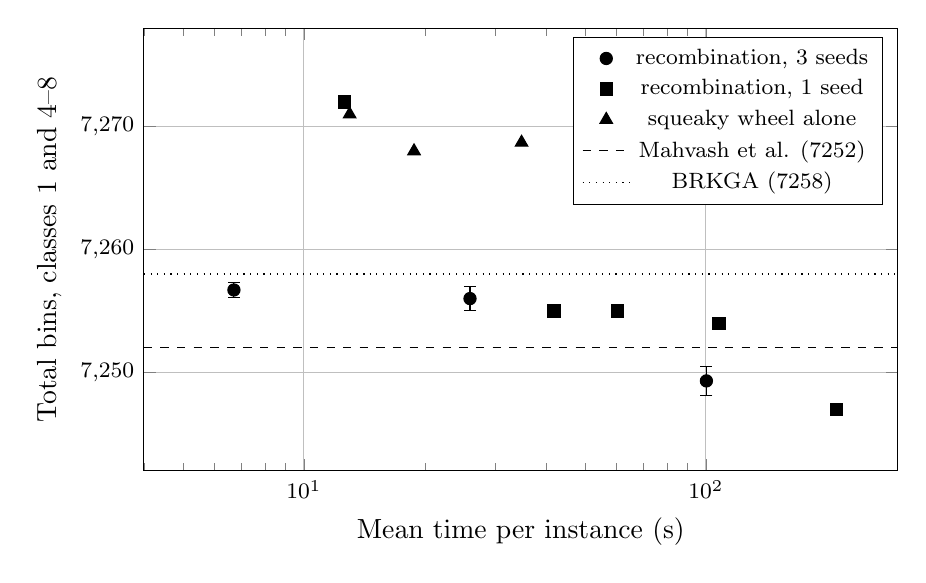
\begin{tikzpicture}
\begin{axis}[width=0.92\textwidth,height=7.2cm,xmode=log,xmin=4,xmax=300,ymin=7242,ymax=7278,
  xlabel={Mean time per instance (s)},ylabel={Total bins, classes 1 and 4--8},grid=major,
  legend style={font=\footnotesize,at={(0.98,0.98)},anchor=north east},tick label style={font=\footnotesize}]
\addplot[only marks,mark=*,mark size=2.2pt,error bars/.cd,y dir=both,y explicit]
  coordinates {(6.7,7256.7) +- (0,0.6) (25.9,7256.0) +- (0,1.0) (100.3,7249.3) +- (0,1.2)};
\addlegendentry{recombination, 3 seeds}
\addplot[only marks,mark=square*,mark size=2.2pt] coordinates {(12.6,7272) (41.9,7255) (60.2,7255) (107.8,7254) (211.3,7247)};
\addlegendentry{recombination, 1 seed}
\addplot[only marks,mark=triangle*,mark size=2.6pt] coordinates {(13,7271) (18.8,7268.0) (34.8,7268.7) (103.7,7267)};
\addlegendentry{squeaky wheel alone}
\addplot[dashed,no marks,domain=4:300] {7252};
\addlegendentry{Mahvash et al. (7252)}
\addplot[dotted,no marks,domain=4:300] {7258};
\addlegendentry{BRKGA (7258)}
\end{axis}
\end{tikzpicture}
\caption{Total bins against mean time per instance on the 240 original instances. Circles: \cfgfast{}, \cfgbal{}
and \cfgqual{} (three seeds, bars: standard deviation; all three from the campaigns of November 2026). Squares, one seed: budget 10 s with recombination
limit 20 s, a run with $T=33$ s and $T_{\mathrm{milp}}=60$ s, and runs of $T=50$ and $T=100$ with the harvest, and $T=200$
(Table~\ref{tab:e-budget}). Triangles: squeaky wheel alone with the time given (13, 18.8, 34.8 and 103.7 s; the second
with two seeds, the third with three, the others with one). The horizontal lines are totals from the literature,
whose times are not comparable.}
\label{fig:e-curve}
\end{figure}

Two observations qualify the table. First, the harvest helps with small budgets and not with large ones: with
$T=100$ and the harvest the result (7254, one seed) is above that of \cfgqual{} without it (7249 in that seed of the earlier campaign; worse in 7
instances and better in 2, $p=0.18$), which agrees with the explanation that a larger pool makes the MILP harder under a fixed time
limit. Second, the runs with one seed are subject to the variation between seeds, whose standard
deviation on the total is 0.6, 1.0 and 1.2 bins for \cfgfast{}, \cfgbal{} and \cfgqual{} (and 3.5 for \cfgfast{} without the harvest, in the repetition); as noted above, the variation
between campaigns can be larger than that.
\paragraph{Time per instance.}
The limits bound the time of the two phases, but the recombination uses time up to its limit in a few runs, so the
mean exceeds the median: \cfgfast{} has a median of 4.2 s, a mean of 6.7 s and a maximum of 34.2 s, and \cfgbal{}
20.5, 25.9 and 80.4 s. The MILP reaches its limit without a proof in 4.6\% to 7.9\% of the runs. Anyone who needs a
bound on the running time should read the maximum, $T+T_{\mathrm{milp}}$ plus one construction. The distribution is in
Table~\ref{tab:e-time} (Appendix~\ref{app:tables}).

\subsection{Comparison with the literature, rotations}
\label{sec:e-rot}

\pend{All the rows of this section come from campaigns whose raw files were lost. Repeat \cfgfast{},
\cfgbal{}, \cfgqual{}, the configuration with $T=33$ and the matched squeaky wheel loop on the 320 instances
with rotations under the protocol of Section~\ref{sec:e-setup}; this is the strongest comparison of the paper.}

With rotations the blocks include the six orientations; nothing else changes. Table~\ref{tab:e-rot} gives the results and the totals of
\citet{Mahvash2018} (Table~1 of their article, sum of the averages of their cells times ten; the total of 6854 for classes 1 and 4--8 is computed by us from their rows, and the
total of 9013 for the eight classes is the one they print) and of BRKGA with six orientations \citep{Goncalves2013}. The BRKGA values for 200 boxes in classes 6, 7 and 8 are below the lower bound with
rotations, which cannot happen for averages of valid solutions of the same instances, so we do not use that total as a reference.

\begin{table}[t]
\centering
\small\setlength{\tabcolsep}{4pt}
\caption{Total bins with rotations (six orientations). Ours: mean and standard deviation over three seeds; time per instance in brackets. All our rows come from earlier campaigns (two to five runs in parallel, raw files not kept), and the rows of different configurations were not run in the same campaign. $^{a}$ Time limit equal to the mean time of the $T=33$ configuration.}
\label{tab:e-rot}
\begin{tabular}{@{}lrrr@{}}
\toprule
Method & Classes 1, 4--8 (240) & Classes 2, 3 (80) & All classes (320)\\
\midrule
Squeaky wheel alone, matched time$^{a}$ & 6845.3 (39 s) & 2165.0 (57 s) & 9010.3\\
\cfgfast{} & $6840.0\pm 1.0$ (7.2 s) & --- & ---\\
\cfgbal{} & $6840.0\pm 3.0$ (26.5 s) & --- & ---\\
$T=33$, $T_{\mathrm{milp}}=60$, without harvest & $6835.3\pm 1.2$ (43 s) & $2159.0\pm 1.0$ (57 s) & 8994.3\\
\cfgqual{} & $6831.0\pm 2.0$ (98.2 s) & $2154.3\pm 0.6$ (117.4 s) & 8985.3\\
\midrule
\citet{Mahvash2018} & 6854 & 2159 & 9013\\
BRKGA, \citet{Goncalves2013} & 6837 (not reliable) & 2172 & 9009\\
\bottomrule
\end{tabular}
\end{table}

\cfgqual{} obtains 8985.3 bins on the eight classes against 9013 of \citet{Mahvash2018}, 27.7 bins (0.31\%) fewer, in 98.2 and 117.4 s per instance against a time per instance
of a few seconds to under 1000 s on their machine (about 310 s on average over the 32 rows of their Table~1). Cell by cell, in classes 1 and 4--8 it is below their total in 12 of the 24 cells, equal in 10 and above in 2; in
classes 2 and 3 it is below in 6 cells and above in 2 (class 2 and class 3 with 200 boxes: 42.13 against 41.9 and 42.17 against 42.1). \cfgbal{} is below in 11, equal in 9 and above in 4
of the 24 cells of the first group. With rotations the larger budget does pay: \cfgqual{} is nine bins below \cfgbal{} in classes 1 and 4--8, better in 10, 12 and 8 instances per seed and worse in 0, 1 and 2
($p=0.0016$, $0.0023$ and $0.058$). The recombination also contributes here: the configuration with $T=33$ is 10.0 bins below the squeaky wheel alone
in classes 1 and 4--8 ($p=0.0027$, $0.0455$ and $0.0075$ by seed), and 6.0 in classes 2 and 3, where the difference per seed is not significant at the 5\% level ($p=0.125$, $0.109$ and $0.065$).
\cfgfast{} also improves on the squeaky wheel alone with rotations (6840.0 against 6845.3) although $\tau=0.005$ s was set for fixed orientation.

\subsection{Contribution of the components}
\label{sec:e-ablation}

\pend{Replace Table~\ref{tab:e-ablation} with the repetition under the protocol
(three seeds, raw files in \texttt{results/bpp/ablation\_2026-11}), which adds a squeaky wheel loop with
$T=26$ s as a control with the same time as the configuration with recombination and harvest. The table is
generated by \texttt{problems/clp/experiments/table\_ablation.py} from the raw files.}

Table~\ref{tab:e-ablation} adds the components one at a time on the 240 original instances with the same search budget
($T=20$ s, $\tau=0.005$ s). The construction with profit $v^2$ (without squeaky wheel) gives 7383.5 bins in 0.1 s per instance; with $\kappa=1$,
that is, maximizing the volume of each bin, it gives 7608.5, and is worse in 151 or 152 of the 240 instances depending on the seed. The squeaky
wheel loop reduces the total by 115.5 bins ($p\approx 10^{-23}$). The learning matters: with $\rho=0$,
where the loop only adds noise, the total is 7307.5, 39.5 bins above the loop with learning. The recombination removes 10 more bins ($p=0.0075$ and $0.0039$
in the two seeds), and the harvest 5.5 more ($p=0.058$ and $0.059$): in this protocol the effect of the harvest is borderline in each seed.
The total reduction from the plain construction to \cfgbal{} is 131 bins, 1.8\%. This ablation is from the earlier campaign, whose raw files were lost; its last row (7252.5) is
3.5 bins below the repetition of \cfgbal{} (7256.0 with the same options), so the effects of the last two components, 10 and 5.5 bins, are reliable only as orders of magnitude;
the effect of the harvest was measured again in the repetition (Table~\ref{tab:e-harvest}).

\begin{table}[t]
\centering
\small\setlength{\tabcolsep}{4pt}
\caption{Ablation on the 240 original instances (fixed orientation, $T=20$ s, $\tau=0.005$ s, two seeds; earlier campaign, raw files not kept).
Each row adds a component to the previous one except the rows marked with $\ast$.}
\label{tab:e-ablation}
\begin{tabular}{@{}lrrrr@{}}
\toprule
Configuration & Bins, seed 1 & Bins, seed 2 & Mean & Time (s)\\
\midrule
Construction, $\kappa=2$ & 7384 & 7383 & 7383.5 & 0.1\\
$\ast$ Construction, $\kappa=1$ & 7613 & 7604 & 7608.5 & 0.1\\
+ squeaky wheel loop & 7269 & 7267 & 7268.0 & 18.8\\
$\ast$ squeaky wheel without learning ($\rho=0$) & 7312 & 7303 & 7307.5 & 19.0\\
+ recombination ($T_{\mathrm{milp}}=60$) & 7259 & 7257 & 7258.0 & 24.4\\
+ harvest ($K=10$, \cfgbal{}) & 7253 & 7252 & 7252.5 & 25.8\\
\bottomrule
\end{tabular}
\end{table}

The effect of the harvest depends on the budget. With the budget of \cfgfast{} (Table~\ref{tab:e-harvest}), adding it to the same configuration
(7266.0 without it) lowers the total to 7256.7, 9.3 bins (0.13\%; $p=0.0002$ on the means of the instances) with 0.9 s more per instance. The squeaky wheel loop alone is not changed
(the totals before the recombination are 7275.0 without the harvest and 7277.3 with it); the whole gain is in the recombination, which removes on average 20.7 bins with the harvest and 9.0
without it. The recombination improves the solution in 8.6\% of the runs with the harvest and in 3.8\% without it. In an earlier campaign with the same
configuration the totals were 7269.7 and 7259.3 (difference $-10.3$; by seed $-14$, $-4$, $-13$). With rotations, \cfgfast{} without harvest obtains $6846.3\pm 3.8$ and with it $6840.0\pm 1.0$ (difference $-6.3$, $p=0.018$;
by seed $-10$, $-1$ and $-8$).

\begin{table}[t]
\centering
\small\setlength{\tabcolsep}{4pt}
\caption{Effect of the harvest at the budget of \cfgfast{} ($T=4$ s, $\tau=0.005$ s, $T_{\mathrm{milp}}=30$ s; 240 original instances; repetition of November 2026).}
\label{tab:e-harvest}
\begin{tabular}{@{}lrrrrr@{}}
\toprule
 & Seed 1 & Seed 2 & Seed 3 & Mean $\pm$ sd & Time (s)\\
\midrule
Without harvest & 7270 & 7264 & 7264 & $7266.0\pm 3.5$ & 5.8\\
With harvest ($K=10$) & 7257 & 7256 & 7257 & $7256.7\pm 0.6$ & 6.7\\
Difference & $-13$ & $-8$ & $-7$ & $-9.3$ & $+0.9$\\
$p$ (Wilcoxon, per seed) & 0.0003 & 0.021 & 0.035 & & \\
\bottomrule
\end{tabular}
\end{table}

Inside the runs of the repetition, comparing the incumbent of the squeaky wheel loop with the final solution,
the recombination removes 8 to 22 bins per seed over the 240 instances, in every seed and configuration ($p<0.005$),
and never worsens a solution (Table~\ref{tab:e-within}, Appendix~\ref{app:tables}). This does not show that its time
is better spent than in the squeaky wheel loop; the matched-time controls of Section~\ref{sec:e-recomb} do.

\paragraph{Parameters of BSG.}
The parameters of BSG were not retuned for bin packing, and the following test shows that the construction does not depend on them. On 120 generated instances (classes 1 and 4--8,
sizes 50 to 200, five instances each) with the construction alone, we varied one parameter at a time: $f_{\min}$ from 0.8 to 1.0, $N_{\max}$ from 100 to 4000, $\alpha$ from 0 to 4, $\beta$
from 0.5 to 4.75, $\gamma$ from 0 to 1 and $p$ from 0 to 0.088. All the totals were within 3 bins of 3649 ($\pm 0.08\%$). We also drew 24 random combinations of all the parameters; the totals
had mean 3649.9, standard deviation 3.0 and range 3645 to 3656, against 3650 for the default values, and the parameters tuned for the ULD problem gave 3653. What changes the result is the choice of the profits (the exponent $\kappa$,
Table~\ref{tab:e-ablation}) and the squeaky wheel loop, not the parameters of the evaluation function.

\subsection{Behaviour of the recombination}
\label{sec:e-recomb}

\paragraph{Effect in several samples.}
Table~\ref{tab:e-milp} compares the squeaky wheel followed by the recombination with the squeaky wheel alone with the same mean time.
The gain is between 10 and 13 bins (0.14\% to 0.43\%) in the samples where the control has about the time of the recombination or, for \cfgfast{} on the first blind set, five times more; on the second blind set the control with four times the time of \cfgfast{} is 6 bins above. Only the classes 2 and 3 and the two blind sets are independent of the design; the
first set of generated instances (240) was used to choose the exponent $\kappa$ and the parameters of BSG (not the budgets of the recombination), and the original
instances decided the configuration. The recombination mixes patterns that the loop itself created, which no iteration of the loop could mix. It does not make a solution worse in the campaigns that we measured, because
it starts from the best solution, but the improvement is rare: in classes 2 and 3 and in the 240 generated instances it saved a bin in 17 of 80 and 17 of 240 instances in at least one seed,
and in 9 to 13 instances per seed.

\begin{table}[t]
\centering
\small\setlength{\tabcolsep}{4pt}
\caption{Total bins of the squeaky wheel alone (``Alone'') and of the squeaky wheel followed by the recombination (``With recomb.''), the first with a time limit close to the mean time of the second except where noted. Each row is one campaign in which the two columns were run
under the same conditions; the campaigns differ from one another (Table~\ref{tab:e-conditions} and the text of Section~\ref{sec:e-setup}), so the rows are compared inside the row and not across rows. The configuration with recombination is
$T=33$ s, $T_{\mathrm{milp}}=60$ s, without harvest, except where noted. $^\dagger$ The result on the original instances was obtained with a prototype in which the
same MILP was solved from Python with HiGHS; the C++ implementation gave 7255 in one seed and the same total in 237 of the 240 instances. In this row the control ran 34.8 s
against 42.8 s for the configuration with recombination; in the other rows with $T=33$ and in the row of \cfgbal{} the times differ by less than 3 s, and in the rows of \cfgfast{} the control ran 35.3 s against 7.3 s (blind set) and 25.3 s against 6.9 s (blind set 2).}
\label{tab:e-milp}
\begin{tabular}{@{}lrrrrr@{}}
\toprule
Sample & Seeds & Alone & With recomb. & Diff. & $p$\\
\midrule
Classes 2 and 3 (80), held out & 5 & 2527.8 & 2517.0 & $-10.8$ & 0.0002\\
Blind set (128), $T=33$ & 3 & 3941.3 & 3930.7 & $-10.7$ & 0.0004\\
Blind set (128), \cfgfast{} & 3 & 3941.3 & 3931.3 & $-10.0$ & 0.0007\\
Blind set 2 (128), \cfgbal{} & 1 & 3893 & 3882 & $-11$ & 0.0010\\
Blind set 2 (128), \cfgfast{} & 1 & 3893 & 3887 & $-6$ & 0.15\\
First generated set (240) & 3 & 7253.0 & 7242.7 & $-10.3$ & 0.0003\\
Original instances (240)$^\dagger$ & 3 & 7268.7 & 7256.0 & $-12.7$ & 0.0001\\
\bottomrule
\end{tabular}
\end{table}

By class (Figure~\ref{fig:e-class}, Appendix~\ref{app:tables}), the gain is concentrated in class 1: in the first set of generated instances the recombination saves 7.0 bins in class 1, 2.0 in class 8, 1.0 in classes 5 and 6, 0.3 in class 7 and none in class 4
(these differences are with respect to the squeaky wheel of 33 s that the recombination starts from). In classes 2 and 3 it saves 6.6 and 4.0.
For the ten instances of class 4 with 50 boxes we enumerated the feasible loads of at most four boxes (checking that
five boxes do not change the result in four instances) and solved the exact cover: it gives 294 bins, the same total as our solver. This suggests that there is nothing to gain in that cell, although we did not prove that no bin can hold more boxes
than the ones enumerated.

\paragraph{Second blind set.}
We measured the recombination on a second blind set of 128 instances (Section~\ref{sec:e-setup}) that we generated for this purpose with registered seeds. Each configuration of
Table~\ref{tab:e-recomb} (Appendix~\ref{app:tables}) was run once on every instance; all the solutions are valid and the raw files are kept. The lower bound of the 128 instances adds up to 3656.

With the budget of \cfgbal{} the recombination lowers the total from 3893 (squeaky wheel alone with the same time) to 3882: $-11$ bins, better in 11 instances and worse in none ($p=0.0010$), a gain
of the size seen in the other samples (Table~\ref{tab:e-milp}). \cfgfast{}, with a quarter of the time, obtains 3887 ($-6$ with respect to the squeaky wheel alone, $p=0.15$), and removing the harvest from it gives 3893 ($+6$, $p=0.11$);
with one seed neither of these two differences is significant. The harvest multiplies the pool by 7.5 (467 to 3493 columns on average).

\paragraph{Cost of the recombination.}
The recombination is cheap in most instances (Figure~\ref{fig:e-outcome}). With \cfgbal{}, the LP of the pool proves in 113 of the 128 runs (88\%) that the pool has no solution with fewer bins than the incumbent, and in 101 of them (79\% of the runs) the first
LP is enough and no MILP is solved. The MILP proves it in nine more runs, so 122 runs (95\%) end with a proof for the pool, and the MILP improves the solution in 12 (9.4\%). In six runs (4.7\%) the MILP reaches its limit of 60 s without a proof
and without an improvement, and they use 54\% of the total time of the MILPs (360 of 661 s). \cfgfast{} behaves in the same way (95\% of the runs proven, 10.9\% improved, 7 unproven runs with 56\% of the MILP time). On 192 instances used during the development,
with the configuration of 33 s, the corresponding figures were 94\%, 12.5\% and 6\%.

\begin{figure}[t]
\centering
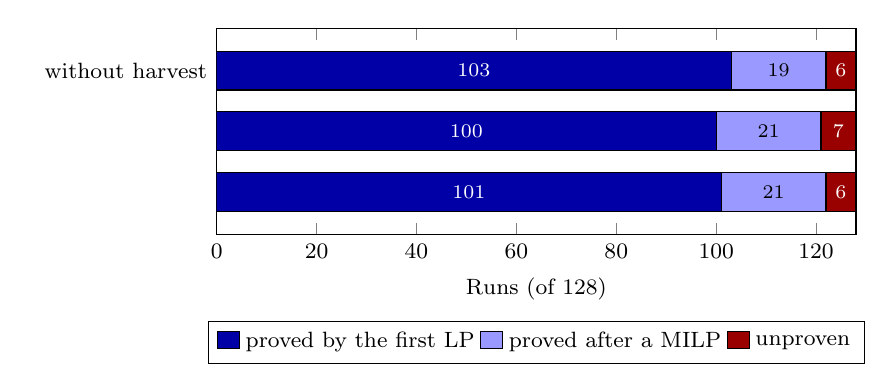
\begin{tikzpicture}
\begin{axis}[xbar stacked,width=0.8\textwidth,height=4.2cm,xmin=0,xmax=128,ytick={0,1,2},y dir=reverse,
  yticklabels={{\cfgfast{} without harvest},{\cfgfast{}},{\cfgbal{}}},xlabel={Runs (of 128)},bar width=14pt,ymin=-0.7,ymax=2.7,
  legend style={font=\footnotesize,at={(0.5,-0.42)},anchor=north,legend columns=3},tick label style={font=\footnotesize},label style={font=\footnotesize},
  nodes near coords,every node near coord/.append style={font=\scriptsize,text=white}]
\addplot[fill=blue!65!black] coordinates {(103,0) (100,1) (101,2)};
\addlegendentry{proved by the first LP}
\addplot[fill=blue!40!white,nodes near coords style={text=black}] coordinates {(19,0) (21,1) (21,2)};
\addlegendentry{proved after a MILP}
\addplot[fill=red!60!black] coordinates {(6,0) (7,1) (6,2)};
\addlegendentry{unproven}
\end{axis}
\end{tikzpicture}
\caption{How the runs of the second blind set end: the first LP of the pool proves that the incumbent is the best of the pool, a MILP is needed and then the LP or the MILP proves it, or the MILP reaches
its time limit without a proof.}
\label{fig:e-outcome}
\end{figure}

The LP of the pool also bounds what a recombination can obtain from its columns. With \cfgbal{}, the sum of the rounded LP values is 3867 and the solutions add up to 3882 bins: in 113 instances the
solution equals the rounded LP value and in 15 it exceeds it by one, so at most 15 bins (0.4\%) could be gained with these pools. The figures are 3873 against 3887 for \cfgfast{} (114 and 14 instances) and 3877 against 3893 for \cfgfast{} without harvest. A better pool, not a better recombination, is
then the way to improve; this agrees with the 0.9\% bound that we obtain on large instances (Section~\ref{sec:e-scale}).

\paragraph{LP bound and reduced-cost fixing.}
The saving of time comes mainly from the LP bound and little from the fixing. A MILP stage was needed in 27 of the 128 runs of \cfgbal{}, and in them the fixing kept on average 86\% of the columns (median 96\%): when the LP
leaves a gap with respect to the incumbent, few columns can be discarded. The plain MILP (warm start, without LP proof and without fixing) with the same budget takes 17.1 s per instance on average against 5.2 s of the version with LP proof and fixing
(total 2190 s against 661 s, $-70\%$), and obtains 3884 bins against 3882. The difference in time is concentrated in the 60 runs in which the plain MILP needs more than 5 s (2107 s against 634 s). The two runs of an instance do not
share exactly the same pool, because the clock changes the search of BSG, so this compares the two procedures and not the two models over one pool. We do not report a separate measurement of the fixing alone.

\subsection{Generalisation: held-out classes and blind sets}
\label{sec:e-heldout}

Classes 2 and 3 were never used to choose a configuration. We ran on them the configuration that we had then
(squeaky wheel of 33 s followed by the recombination with a limit of 60 s, without harvest) and of \cfgfast{}. The
standard deviation of this configuration (1.4) is the sample one, computed from the five totals 2519, 2517, 2515, 2517 and 2517. The
recombination saves 10.8 bins (0.43\%) with respect to the squeaky wheel alone with the same time (Wilcoxon $p=0.0002$ over five seeds); in each
seed it improves 10 to 14 instances and worsens none. This configuration obtains 2517.0, below the totals published for BRKGA (2519), GVND (2527) and TS3 \citep{Lodi2002}
(2543), and above the total of \citet{Mahvash2018} (2514). \cfgfast{} obtains 2521.0, four bins above the longer configuration, with 5.4 times less
time. We did not run \cfgbal{} and \cfgqual{} on these classes without rotation.

The blind set confirms the two effects. \cfgfast{} (3931.3) is 0.7 bins above the configuration with $T=33$ (3930.7, $p=0.16$) with five
times less time, and both are about ten bins below the squeaky wheel alone with the time of the second (3941.3):
$-10.0$ ($p=0.0007$) and $-10.7$ ($p=0.0004$). Removing the harvest from \cfgfast{} raises the total by 4.7 bins ($p=0.011$ on the means of
the instances; per seed $+4$, $+5$, $+5$ with $p=0.046$, $0.096$ and $0.025$). That is a smaller effect than on the original instances (below).

\subsection{Vertical support: industrial instances}
\label{sec:e-ind}

\pend{The large instances use the construction alone, as when the recombination was believed to be incompatible
with support. With the partitioning model the whole pipeline applies: run, at the same time per instance
($\approx 18$ s and $\approx 60$ s), the construction alone with $\tau=2$ s against the squeaky wheel loop with
$\tau\in\{0.2,0.5\}$ s, with and without the partitioning recombination. The instances, their converter and the
support validator must be added to the repository.}

\paragraph{Configuration.}
These instances have 50 to 2000 boxes and bins that hold more than a hundred boxes when $n\ge 500$. We require, on every box above the floor, that at least 70\% of its
base rests directly on boxes (Section~\ref{sec:m-ext}). In the runs reported here, for $n\ge 500$ we use the construction alone, with $\kappa=1$ and $\tau=2$ s per bin.
These values were chosen by looking at a few instances of this benchmark (the first instance of each class with $n=1000$, the second instance of classes 1 and 2 with $n=500$, the first instance of class 1 with $n=500$ and 2000 and eight
instances of classes 3 and 4 with $n=1500$ and 2000); the choice is not independent of the benchmark.

\paragraph{Comparison with LCGA.}
Table~\ref{tab:e-ind} gives the mean number of bins per cell for $n\ge 500$, with one run per instance, against the values of \citet{Elhedhli2019} (Table~9 of their article). The total over the 16 cells is 144.6 bins against 153.6 (5.9\% fewer):
we are below in 11 cells, equal in 5 and above in none (exact sign test, $p=0.0010$; the cells share a configuration and a choice of parameters, so the test is descriptive). Three runs of the whole set (the construction is deterministic except for the clock) gave 723, 721 and 723 bins in the 80 instances,
that is, 722.3 on average (144.5 as a sum of cell means), and in each run 80 of 80 solutions satisfy the 70\% support in every box (independent check of geometry and support). The time per instance is 18.3 s on average with two runs in parallel, against 608 s for LCGA;
that is 33 times less in raw time and about 15 times after a factor of 2.27 between the single-thread ratings of the two processors \citep{PassMark} (3740 for the i5-14400 and 1650 for the i7-5500U; the factor is approximate). In the instances 3 to 5 of each cell, which were not looked at while choosing $\kappa$ and $\tau$, the excess over the lower bound
is 0.92 bins per instance for our method and 1.46 for LCGA (compared by cell averages because the numbering differs).

\begin{table}[t]
\centering
\small\setlength{\tabcolsep}{4pt}
\caption{Industrial instances, $n\ge 500$: mean number of bins per cell (five instances), ours with one run per instance and two runs in parallel at below-normal priority (construction alone, $\kappa=1$,
$\tau=2$ s, support 70\%) and LCGA \citep{Elhedhli2019}.}
\label{tab:e-ind}
\begin{tabular}{@{}lrrrrrrrr@{}}
\toprule
 & \multicolumn{4}{c}{Ours} & \multicolumn{4}{c}{LCGA}\\
\cmidrule(lr){2-5}\cmidrule(lr){6-9}
Class & 500 & 1000 & 1500 & 2000 & 500 & 1000 & 1500 & 2000\\
\midrule
1 & 4.0 & 8.2 & 12.0 & 16.0 & 5 & 8.8 & 12.4 & 16\\
2 & 4.0 & 8.0 & 12.0 & 16.0 & 5 & 9 & 12 & 16\\
3 & 4.0 & 7.0 & 10.0 & 13.0 & 4 & 7 & 10.6 & 14\\
4 & 3.4 & 6.0 & 9.0 & 12.0 & 4 & 7 & 10 & 12.8\\
\midrule
Sum & \multicolumn{4}{c}{144.6} & \multicolumn{4}{c}{153.6}\\
\bottomrule
\end{tabular}
\end{table}

Three caveats limit this comparison. The instances are from the same distribution but we could not verify that they are those of the article. The support: LCGA does not impose it on every box in its main results; its columns of supported items
in the appendix tables give 78.2\% of the boxes with at least 70\% support (83.2\% for $n\ge 500$) and a mean support of 92.3\% for $n\ge 500$ (our reading of their tables), while we impose 70\% on every box and obtain a mean support of 90.5\% to 92.6\%. This
makes our requirement the stricter one. Last, \citet{Elhedhli2019} allow a tolerance of 5 mm in the heights when forming layers, and we require exact contact.

\paragraph{Time per bin and $\kappa$.}
On the 48 instances obtained by resampling and the 24 from the catalogue (Table~\ref{tab:e-indnew}, Appendix~\ref{app:tables}), the default configuration for the Martello et al.\ instances ($\kappa=2$, $\tau=0.02$ s) gives 497 and 264 bins; the
configuration of this section ($\kappa=1$, $\tau=2$ s) gives 438 and 233, 11.9\% and 11.7\% fewer, but with 18 s per instance instead of less than one second. The fair control is the one that keeps $\tau=2$ s and
$\kappa=2$: it gives the same 438 bins in the resampled instances (4 instances better, 4 worse, 40 equal) and 241 in the catalogue instances, eight bins more (3.3\%) than $\kappa=1$ (better in 8, worse in none). Most of the gain thus
comes from the time per bin, and $\kappa=1$ helps only in the catalogue instances.

\paragraph{Cost of the support requirement.}
Table~\ref{tab:e-support} shows the construction with $\kappa=1$ and $\tau=2$ s on the 80 instances with $n\ge 500$ for several support criteria. Requiring 70\% on every box costs 15 bins out of 708 (2.1\%) with respect to requiring nothing; without a requirement, only 77.3\% of
the boxes have 70\% of support, so the explicit condition is necessary. Stricter criteria are costly: 85\% costs 9.7\% more than 70\%, and full support 80\% more. We
also tried 95\% and 100\% of the base on eight instances (classes 1--4, first instance, $n=500$ and 1000): 43\% and 89\% more bins than 70\% (the total of the eight was 63 and 83 against 44), so the cost does not appear only with full support. We did not determine whether the block structure of the
generator or the criterion itself is the cause.

\begin{table}[t]
\centering
\small\setlength{\tabcolsep}{4pt}
\caption{Criteria of support (industrial instances, $n\ge 500$, 80 instances, construction alone, $\kappa=1$, $\tau=2$ s, one run per instance, two runs in parallel). Support: percentage of the base area resting on boxes.}
\label{tab:e-support}
\begin{tabular}{@{}lrrrrr@{}}
\toprule
Criterion & Bins & Time (s) & Mean support & Boxes with $\ge 70\%$ & Boxes fully supported\\
\midrule
None & 708 & 17.3 & 80.4\% & 77.3\% & 28.3\%\\
50\% of the base & 720 & 17.9 & 88.7\% & 86.9\% & 32.6\%\\
70\% of the base (used) & 723 & 18.3 & 91.4\% & 100\% & 33.0\%\\
85\% of the base & 793 & 19.6 & 95.2\% & 100\% & 37.2\%\\
Full support & 1303 & 32.1 & 100\% & 100\% & 100\%\\
\bottomrule
\end{tabular}
\end{table}

\paragraph{Small industrial instances.}
For $n<500$ the construction alone leaves one or two bins per cell and is not better than LCGA (23.4 against 23.0 bins over the 16 cells). With a configuration that also includes the improvement phase of Appendix~\ref{app:improve}
($T=30$ s, 30\% of it for the squeaky wheel loop and the rest for the improvement phase, with the reload from scratch, $\kappa=1$,
$\tau=0.02$ s in the construction and 0.04 s in the improvement phase) the total is 22.0 against 23.0 (below in two cells and equal in 14), with 5 s per instance on average because the search stops when the lower bound is reached.

\subsection{Limits: large instances}
\label{sec:e-scale}

The recombination does not scale to instances with several hundred boxes with the budgets used here. On 36 generated instances with $n=500$ and $n=1000$ (six classes, three instances per class and size), the squeaky wheel followed by the recombination (50 s and 60 s) obtains 6183 bins in 101.5 s,
against 6179 of the squeaky wheel alone with 102 s (the second is better in 5 instances and the first in 1, $p=0.22$). The recombination improves one instance of 36, uses the whole limit of 60 s in almost all of them (50.0 s on average) and works with about 2095 columns.
The lower bounds are 1955 for $n=500$ and 3958 for $n=1000$, against 2056 and 4127 bins of the first configuration. In another set of 24 generated instances (six classes, two sizes with $n=500$ and 1000, two instances each), the pools of \cfgbal{} give
4072 bins, and the sum of the rounded LP values of those pools is 4036: even a perfect recombination of those pools could save at most 36 bins (0.9\%). The margin
is then in the generation of better columns and not in the recombination.

\subsection{Discussion and limits of the evidence}
\label{sec:e-discussion}

\paragraph{What the results support.}
The recombination of the bins produced by the search is the component that is best supported. In the seven comparisons of Table~\ref{tab:e-milp} the squeaky wheel loop alone has a total that is between 6 and 13 bins above that of the
configuration with recombination, including the comparisons in which the control runs four to five times longer than \cfgfast{}, and inside the runs of the repetition the recombination saves bins in every seed and configuration without ever worsening a solution.
Classes 2 and 3 and the two blind sets were not used to take any decision. Without rotations the total of \cfgfast{} and \cfgbal{} is at the level of the best published ones and that of \cfgqual{} is 2.7 bins below the lowest (7249.3 against 7252), and with rotations the long configuration is below the total of \citet{Mahvash2018}.
In the industrial instances the construction alone, with the 70\% support imposed on every box, uses fewer bins than the totals that \citet{Elhedhli2019} report.

\paragraph{Comparison with the literature.}
The totals of the other methods are taken from their articles. They come from other machines and from an unknown number of runs, and \citet{Mahvash2018} do not report times for the experiments without rotation. We normalised the times only
in the industrial comparison, and with a processor rating that is approximate (Section~\ref{sec:e-ind}), so the statements about time with respect to other methods are indicative. We could not apply statistical tests against the literature because the results per instance
are not published. The total of \citet{Mahvash2018} remains below the shorter configurations without rotation. \cfgqual{} is 2.7 bins below it, with a standard deviation of 1.2 bins over seeds and a different machine, and for that reason we do not claim that the method improves the state of the art in that setting.

\paragraph{Variation between campaigns.}
Repeating \cfgfast{} and \cfgbal{} on the original instances with the same code and options gave totals that differ from those of the earlier campaign by 2.6 and 3.0 bins (Section~\ref{sec:e-mpv}), more than the standard deviation between seeds inside a campaign (0.6 to 2.1 bins); \cfgqual{}, in contrast, moved by 0.7 bins (7250.0 against 7249.3).
Because the time limits are wall-clock limits, the load of the machine changes the amount of search that a run receives, and we do not control it. For this reason, differences of a few bins between configurations measured in different campaigns should not be interpreted, and we
mark the figures that come from campaigns whose raw files were lost.

\paragraph{Tuning on the benchmark.}
The exponent $\kappa$ and the budgets were chosen with the original instances and with generated instances of the same distribution. The absolute totals on the original instances are therefore not independent of the design. The effects that matter for the conclusions
were also measured on classes 2 and 3 and on two blind sets, and they have the same sign and a similar size there. In the industrial instances $\kappa$ and the time per bin were chosen with a few instances of the same benchmark, and the 48 additional instances
were obtained by resampling its boxes, so they are not independent either (Section~\ref{sec:e-ind}).

\paragraph{Limits of the method.}
The recombination does not scale to several hundred boxes with the budgets used here: with $n=500$ and $1000$ it improved one instance of 36, and the LP of the pools shows that at most 0.9\% could be gained from them (Section~\ref{sec:e-scale}). The covering model is not compatible with the support requirement,
because removing the surplus boxes can leave a box without support; the partitioning model is, but its effect on the industrial instances is not measured yet, and the results reported for $n\ge 500$ come from the construction alone. The support criterion is expensive when it is made stricter: 85\% of the base costs 9.7\% more bins than 70\%, and full support 80\% more (Table~\ref{tab:e-support}).
The method needs a MILP solver for the recombination; without it only the construction and the squeaky wheel loop are available.

\paragraph{Industrial instances.}
The industrial totals are the mean of five instances per cell with one run per instance. Three complete runs of the 80 instances with $n\ge 500$ gave 723, 721 and 723 bins, so the variation caused by the clock is small: four instances of the 80 changed by one bin between runs,
and the advantage of 5.9\% over LCGA is much larger than that. The instances have the distribution and the structure of those of \citet{Elhedhli2019}, and the lower bound of their cells coincides with ours in 30 of 32, but we could not verify that they are the same
files, and \citet{Elhedhli2019} tolerate 5 mm in the heights when they form layers while we require exact contact.
